\chapter{Laozi et le Daode jing}

\subsection{Laozi}
\paragraph{Disparate et complexe}

\paragraph{Laozi, personnage légendaire} Cité dans un ouvrage du IV av JC. Au II av JC, la première biographie. 



Laozi, un personnage largement légendaire


Éléments principaux de la légende concernant Laozi:
\begin{itemize}
    \item  	Il aurait eu pour nom Li, pour prénom Er
    \item 	Il aurait été archiviste ou annaliste-devin de la dynastie Zhou
    \item 	La visite que Confucius lui aurait rendue
    \item 	Son exil vers l’ouest à dos de buffle
    \item 	A 50 ans, il arrive sur un buffle noir. Le gardien est content. Il demande à Laozi de coucher son enseignement. Sa rencontre avec Yin Xi, le gardien de la passe, qui lui demanda de coucher par écrit sa doctrine, le classique de le \textit{voie et de la vertu}
\end{itemize}




\begin{marginfigure}
    \centering
        \caption{Laozi sur le buffle Zhang Lu (1490-1563)}
    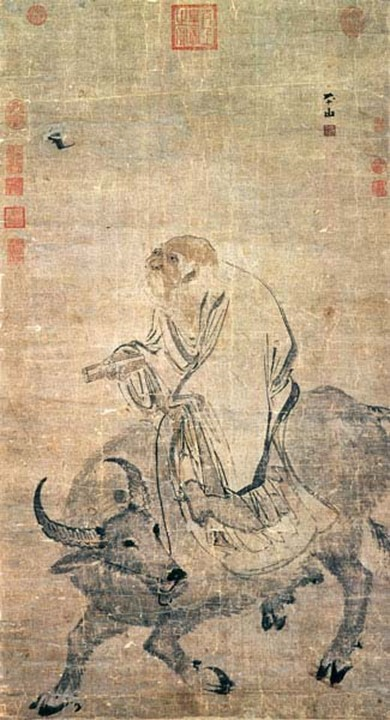
\includegraphics[width=\textwidth]{ConfucianismeTaoismeBouddhismeChinois/Images/Laozi.jpg}

    \label{fig:enter-label}
\end{marginfigure}



\paragraph{L'Ouest} Théorie qui arrive au IIè siècle selon lequel il voulait aller en Inde devenir un Bouddha.



 \subsection{Le Laozi ou le Daode jing }

\paragraph{81 chapitres courts en deux parties} 
une première partie, \textit{classique du Dao / voie} et une deuxième partie, \textit{classique} (jing) de la vertu (\textit{de}). l'ensemble s'appelle le Laozi, traité de la voie et de la vertu.

\paragraph{titre assez tardif} Au moment de la divination, 50 de notre ère. Le mot \textit{jing} signifie le classique. Au plus tard, au 8èùme siècle, le titre devient définitif. Avant, il s'appelait le \textit{Lao}, du nom de leur auteur. 

\paragraph{origine mystérieuse} probablement pas transmission orale car trop complexe. 

\paragraph{Le Laozi ou le Daode jing} : texte attribué à Laozi mais de nature fondamentalement \textbf{composite} (pas une seule personne, une compilation) dont l’origine reste un mystère
\begin{itemize}
    \item 	La version canonique (manuscrit du 3ème siècle avant JC) : 
    \begin{itemize}
        \item Commentaire de Heshang Gong (Vénérable du bord du Fleuve, 170-156 ?) : premier commentaire. POssible qu'il ait découpé aussi en 81 chapitres. Plutôt orientation pratique.
        \item commentaire de Wang Bi (220-265) : important dans l'histoire intellectuelle chinoise car il a aussi commenté le livre des mutations et les entretiens de Confucius. Il fait apparaitre les liens entre les deux documents, assez novateur. Wang Bi a aussi créé l'école des mystères, une branche du taoisme.  Plutot orientation philosophique. 
        
    \end{itemize}

    \item 	Les versions de Mawangdui (manuscrit trouvé dans les combes)

    \item 	Les versions de Guodian (idem)
\end{itemize}


\paragraph{numérologique}
\begin{Prop}[81]
    Correspond à la totalité du cosmos dans la tradition chinoise. Chiffre parfait.  
\end{Prop}


\subsection{Le manuscrit de Mawangdui}

\paragraph{Manuscrit trouvé dans la tombe à Mawangdui} , près de la ville de Changsha, capitale de la province du Hunan actuelle, dans les années 70. 

 \begin{marginfigure}
    \centering
        \sidecaption{Un groupe de tombes datant du début des Han occidentaux (202 av. J.-C.– 9 apr. J.-C.) découvertes à Mawangdui}
    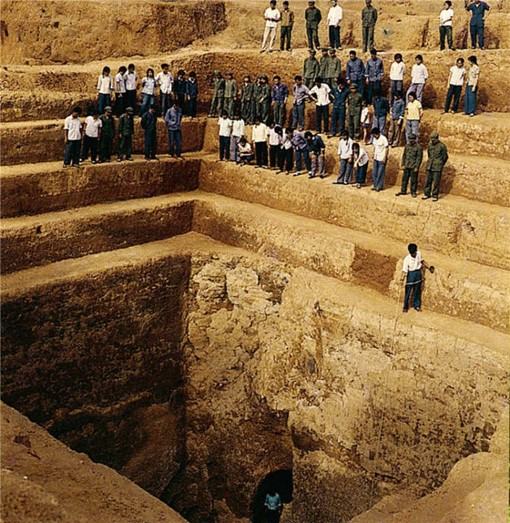
\includegraphics[width=\textwidth]{ConfucianismeTaoismeBouddhismeChinois/Images/tombelaozi.jpg}

    \label{fig:enter-label}
\end{marginfigure}

\paragraph{Biographie dans la tombe }On a trouvé la momie du Seigneur et sa biographie. Il aimé lire ces textes. Cinquantaine de textes et cartes géographiques,, philosophie, médecine, astronomie... 2 versions du Laozi.

 


 \begin{figure}[!h]
    \centering
        \sidecaption{Fragments de la version A du Laozi trouvés dans la tombe n° 3 de Mawangdui. Cette tombe, datant de 168 av. J.-C., appartenait à Li Xi, fils de la marquise de Dai.}
    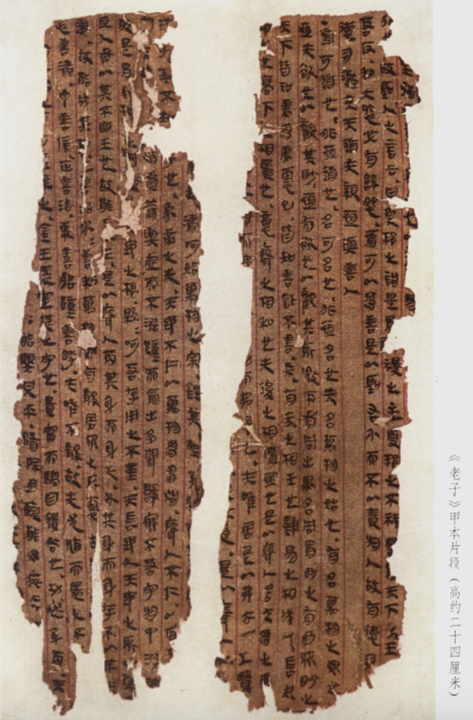
\includegraphics[width=0.5\textwidth]{ConfucianismeTaoismeBouddhismeChinois/Images/Laozitexte.png}

    \label{fig:enter-label}
\end{figure}
\paragraph{comparaison avec la version canonique} des différences, nuances, pas de divergences. Le style est plus dépouillé et clair que la version canonique : elle doit être plus proche du texte d'origine. 


 \subsection{version du Guodian}

 \paragraph{aussi au Sud de la Chine (fleuve Bleu)}

 \paragraph{Tombe}
Tombe n°1 de Guodian, datant du début du 4ème siècle av. J.-C., faisait partie d’un cimetière de l’ancienne capitale de la principauté de Chu, dans la province du Hubei actuelle. Elle a été découverte en 1993.

\paragraph{principauté de Chu} 
   
 
Les Etats indépendants avant l’unification de l’empire en 221 avant notre ère
  
\paragraph{lamelles de bambous} Manuscrits découverts dans la tombe n° 1 de Guodian. 

\paragraph{versions du Laozi}On a trouvé trois versions du Laozi. Ce qui est spécifique, c'est que ces trois versions ne se recoupent pas. L'ordre d'assemblage des textes n'est pas le mêmes entre versions. On peut donc choisir les chapitres qui nous intéresse. Au 4eme siècle av JC, il n'y a pas une version définitive ce qui permet de déduire que c'est uniquement au 3ème siècle qu'il y a une canonisation du texte.


\subsection{importance de l'Ecriture}

 
\paragraph{Taoisme : une doctrine, un culte}

\paragraph{l'Ecriture a une fonction sacrée} Dieu apparait et lui transmet les documents d'investiture. 

\paragraph{Arrivée du Bouddhisme} Pour faire face du Bouddhisme, le taoisme commence à produire des textes (4-5ème siècle de notre ère). Remettre au gout du jour les textes anciens. Ecrivent des codes moraux, instructions rituelles. Apocalypses et prophéties. 

\paragraph{influence bouddhique} bouche de la divinité (influence bouddhique).  Parsonnification du Tao. 

\paragraph{inventaire des textes taoistes au V après JC} Grâce à ces textes, reconnaissance par l'empereur et l'aristocratie. 



\subsection{La bureaucratie céleste}


\paragraph{role missionnaire du Taoisme} Tout un panthéon, construit au cours du temps. 

\paragraph{une bureaucratie céleste en extension} "2000 ans de bureaucratie" en Chine. 

\paragraph{personnification du Tapo} des dieux qui représentent les astres, les étoiles,...

\paragraph{au sommet, les 3 purs, manifestation du Tao} Il y a aussi des personnes réelles qui ont atteint l'immortalité, comme le Seigneur de Fengdu. 



 \begin{figure}[!h]
    \centering
        \sidecaption{À droite: « Le vénérable céleste du commencement originel »
Vers 1700 Musée Guimet; À gauche: « Le seigneur de Fengdu (les enfers taoïstes) et ses six ministres devenus immortels » Vers 1600
Musée Guimet}
    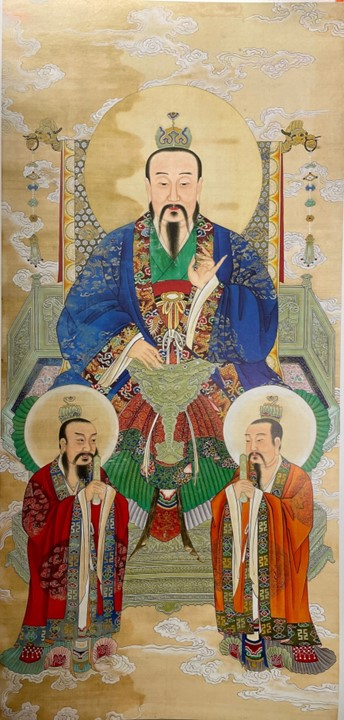
\includegraphics[width=0.4\textwidth]{ConfucianismeTaoismeBouddhismeChinois/Images/Levénérablecélesteducommencementoriginel.jpg}
    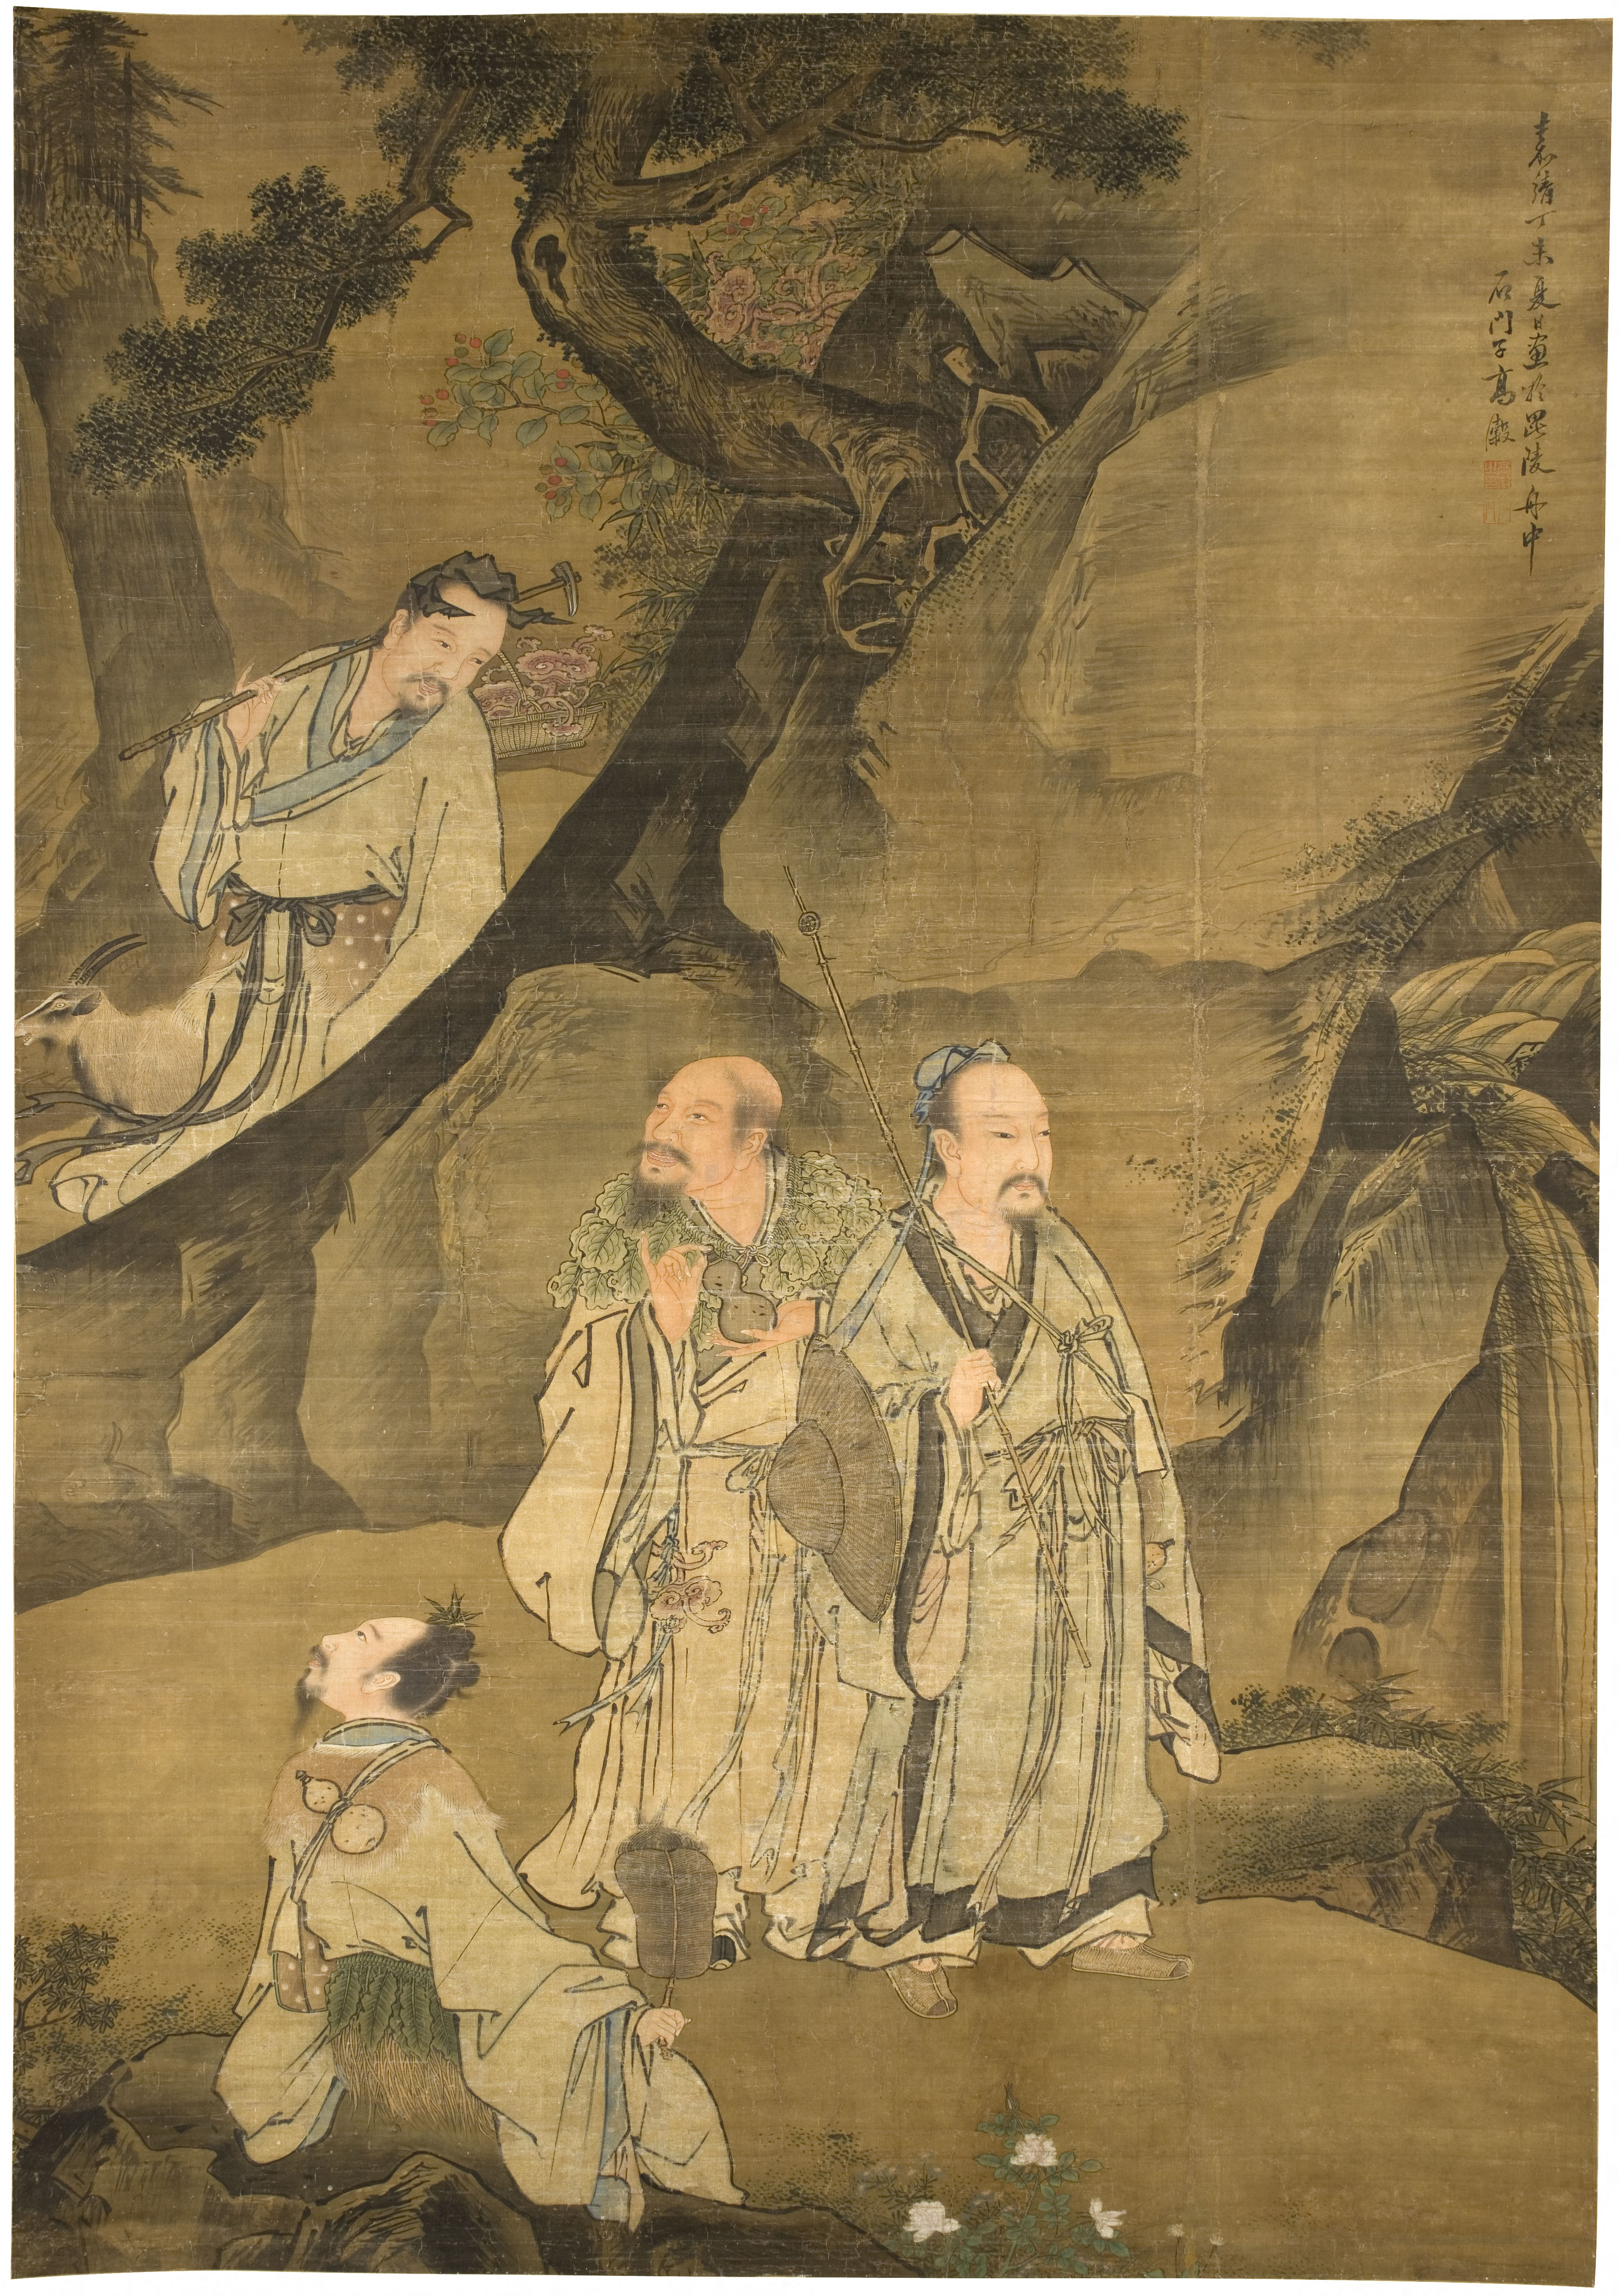
\includegraphics[width=0.54\textwidth]{ConfucianismeTaoismeBouddhismeChinois/Images/Immortels.jpg}
    \label{fig:enter-label}
\end{figure}







%----------------------------------------------------------------
\section{Laozi}



Versions citées :
Anne CHENG, Histoire de la pensée chinoise, Paris : Seuil, 1997.
Rémi MATHIEU (trad.), Le Daode jing « Classique de la voie et de son efficience », Paris : Éditions Médicis- Entrelacs, 2008.


\paragraph{langage assez particulier} le langage est un obstacle, le Dao ne peut être décrit par le langage. \textit{Paradoxe}. Il n'y a jamais de façon systématique, directe de définir la voix. 

\paragraph{des propos paradoxaux} donne confusion. Ne pas rester aux mots, ce ne sont pas des concepts. 

\paragraph{Trois grilles de lecture} \begin{itemize}
    \item politique (il parle du pays),     \item philosophique (il parle de la réalité du monde)     \item et physiologique (un guide des actions et des pratiques).
\end{itemize}
Le salut joue aux trois échelles, entre le microcosme et le macrocosme, entre le pays et le corps. 

\begin{Ex}[Corps]
    Le corps peut être son propre corps ou un pays.
    et inversement, gouvernement du pays : peut être lu comme la préservation de son propre corps.
\end{Ex}


\paragraph{dissoudre les idées reçues pour atteindre les idées plus profondes}


\section{La Voie (le Dao)}

\begin{singlequote}
    1.	La voie que la voix peut dire n’est jamais la constante voie. \\
Le nom que le nom peut nommer n’est jamais le constant nom. \\ Le sans-nom est le commencement du ciel et de la terre.\\
Le qui-a-nom est la mère des dix mille êtres.\\
C’est pourquoi qui est constamment dépourvu de désir  \\fait en sorte d’en contempler les subtilités.\\
Qui est constamment dans l’avoir du désir  \\fait en sorte d’en contempler les manifestations.\\
Ces choses ont, en fait, une même souche, quoiqu’elles aient des noms différents.  \\Semblablement, on les nomme mystérieuses.\\
Pourtant, s’il est encore plus mystérieux que ce mystère,  \\C’est bien la porte qui ouvre sur toutes les subtilités.\\
-- chapitre 1, traduction de Rémi Mathieu, p. 81.
\end{singlequote}

Le tout premier passage du \textit{Taozi} dans la version canonique. 
On doit passer par le \textit{nom}, mais qui ne sont pas constants : impossibilité de dire la chose.
Il y a une réalité première (sans nom, invisible, caché) qui est à la source d'une réalité concrète qui a elle un nom.
On peut comprendre cette réalité première comme le chaos originel, antérieur à la conscience du sujet. 

\begin{Prop}[Le monde]
    le Dao vit dans les deux niveaux, premier et caché, et concret et immanent, les deux réalités du monde. 
    Le Dao peut correspondre à  la vérité. 
\end{Prop}


\begin{singlequote}
    2.	Il est un être formé dans le chaos  \\Né avant Ciel et Terre \\
Silence ! Vacuité ! \\
Il se tient seul, inaltérable Circulant partout sans s’épuiser \\ On peut y voir la Mère du monde \\
Ne connaissant pas son nom, je l’appelle Dao  \\ À défaut d’autre nom, je le dirais grand  \\Grand pour dire qu’il s’écoule \\
S’écoulant, il s’étend au loin \\
À l’extrême lointain, il fait retour  \\Ainsi grand est le Dao \\
Grand est le Ciel Grande est la Terre \\
Comme l’est le souverain des hommes  \\Il est au monde quatre grands \\
Le souverain est l’un d’eux  \\L’Homme prend modèle sur la Terre  \\La Terre sur le Ciel \\
Le Ciel sur le Dao \\
Et le Dao sur ce qui va de soi\sn{ce qui va de soi : ainsi, ce qui est spontané. Ce \textit{truc}, je l'appelle Dao}. \\
-- chapitre 25, traduction d’Anne Cheng, p. 206.
\end{singlequote}

On voit ici les différents niveaux du Dao : au niveau du monde mais de chaque être.
Il évoque le mot \textit{mère} du monde : La création, une action toujours en cours. 
\textit{s'écouler}, elle est toujours en \textbf{mouvement}, fait partior de cette force. Elle ne stagne pas, elle n'est pas inerte, elle ne tarit pas. 

\paragraph{les choses de la nature ont des vertus qui doivent être imités par l'homme} caractéristique de la pensée chinoise.
\begin{Ex}[puissance de la marche du ciel]
Confucius dans le livre des mutations, parle de la puissance de la marche du ciel, et l'homme de bien consolide sa puissance et porte tous les êtres.
\end{Ex}

\paragraph{Taoisme : valorisation du féminin} réceptif, passive, négation, réception : importance de la \textbf{Terre}, qui supporte tout, position très basse mais en même temps, elle pénètre toutes les choses.

 \begin{singlequote}
     3.	Le dao génère l’un. \\
L’un génère le deux. \\ Le deux génère le trois. \\
Le trois génère les dix mille êtres. \\
Les dix mille êtres s’adossent au yin et embrassent le yang ; \\Combinant les souffles du vide, il fait en sorte qu’ils s’harmonisent.\\ Ce que les gens détestent
\\C’est avant tout d’être un pauvre orphelin, dépourvu de vertu, ou un homme sans qualités. \\Pourtant, les rois et les ducs se servent de ces termes pour s’appeler. \\
 C’est pourquoi un être s’avantage parfois en se diminuant \\ Et se diminue parfois en s’avantageant. \\
Ce que les gens enseignent, je l’enseigne moi-même : \\
Celui qui use de force et de violence n’obtient pas de mourir naturellement. \\Je veux considérer cela comme le précepteur de mon enseignement. \\
-- chapitre 42, traduction de Rémi Mathieu, p. 156.
 \end{singlequote}

Passage relativement clair. 10 000 êtres : tous les êtres. 
Les \textit{3 purs} reprennent cette idée de 3. 3 forces à l'origine du monde.
Les dieux ont ils une volonté ? En fait, ils s'identifie tellement au Tao qu'ils n'ont pas réellement de volonté propre.
\paragraph{souffle, manifestation du Dao}

\paragraph{Yin et Yang} l'homme préfère toujours l'action à l'inaction.  Attitude biaisée pour le Taozi qui recommande de voir les deux dimensions. 
Force et faiblesse. Pas toujours aussi simple qu'on le pense. Ainsi, un prince cherchera l'humilité, et ne se mettra pas en avant. 


\section{Renversement ou retour}

\begin{singlequote}
    4.	Atteindre aux limites du vide ; Préserver le comble de la sérénité.\\
Lorsque les dix mille êtres surgissent ensemble, \\Je fais en sorte de contempler leur retour.\\
Or, les êtres sont là à foison,\\
Et chacun d’eux s’en retourne à nouveau à sa racine. \\S’en retourner à sa racine, c’est ce qu’on appelle sérénité ; \\Cela veut dire retourner à son destin.
Retourner à son destin, c’est ce qu’on appelle constance. \\Connaître la constance s’appelle lucidité ;\\
Ignorer la constance, c’est, tel l’insensé, faire surgir le funeste. \\Connaître la constance, c’est être réceptif.\\
Être réceptif, c’est justement être impartial. \\Être impartial, c’est justement être souverain. \\Être souverain, c’est justement être céleste.\\
Être céleste, c’est justement être la voie.\\ Être la voie, c’est atteindre à la pérennité,\\
C’est, de toute sa vie, ne plus jamais se mettre en péril.\\
\textit{ \small -- chapitre 16, traduction de Rémi Mathieu, p. 106.}
\end{singlequote}

Il faut se placer à l'origine pour retrouver la puissance organisatrice de l'univers.
le problème c'est que l'homme est diverti. Retourner à la sérénité pour retrouver le \textit{Dao}. C'est là que l'homme retourne à son destin, \textit{sa nature} conférée par le ciel. Le destin de chacun, c'est le \textit{Dao.}
\paragraph{changement} Rien ne stagne, tout est en constant changement. Le Yin et le Yang bouge, mais si on accède à la réalité première, alors on arrive à la constance véritable. Ne jamais se mettre en péril : une fois qu'on est lié au Dao, on accède à l'immortalité, car le Dao est la seule chose stable dans le monde.

\paragraph{Recherche par les chinois de la longue vie}

\begin{singlequote}
    5.	Les cinq couleurs aveuglent les yeux des hommes. \\Les cinq notes assourdissent les oreilles des hommes. \\Les cinq saveurs gâtent le palais des hommes.\\
Les galops débridés des chasses affolent le cœur des hommes.\\ Les biens rares entravent l’activité des hommes.\\
C’est la raison pour laquelle l’homme saint agit sur les ventres, \\Mais il n’agit pas sur les yeux.\\
Aussi rejette-t-il ceci et prend-il cela.
-- chapitre 12, traduction de Rémi Mathieu, p. 99.
\end{singlequote}

Les 5 notes : toutes les couleurs. 
Il est epuisé par la stimulation de l'environnement. Pour cela, besoin de retourner vers l'intérieur.
Plusieurs interprétations possibles : 
\begin{itemize}
    \item au troisième siècle, commentaire : ventre : centre de la nutrition, besoins essentiels. Et éviter de susciter
    \item une autre explication possible : plus tard !
\end{itemize}


\begin{singlequote}
    6.	Le retour, c’est le mouvement même du Dao \\Le faible, c’est l’efficacité même du Dao \\
Les dix mille êtres sous le Ciel\\ naissent de l’il-y-a\\
Et l’il-y-a naît de l’il-n’y-a-pas.\\
-- chapitre 40, traduction d’Anne Cheng, p. 207.
\end{singlequote}

\paragraph{il n'y a pas } chaos originel. vs \textit{il y a}, ce qui a une forme.  Retourner à l'origine, c'est là qu'on est proche du Dao



\subsection{souplesse du bébé}
\begin{singlequote}
    7.	À sa naissance, un homme est souple et faible ; \\Mais à sa mort, il est rigide et raide.\\
À leur naissance, [parmi les dix mille êtres], les végétaux sont souples et frêles ; \\Mais à leur mort, ils sont secs et flétris.\\
C’est pourquoi ceux qui sont rigides et raides sont des disciples de la mort. \\Tandis que ceux qui sont souples et frêles sont des disciples de la vie.\\
C’est la raison pour laquelle la raideur des armes n’amène jamais la victoire \\Et la rigidité des arbres amène leur brisure.\\
La rigidité et la grandeur se situent en dessous,\\
Tandis que la souplesse et la fragilité se situent en dessus.\\
-- chapitre 76, traduction de Rémi Mathieu, p. 216.
\end{singlequote}

\paragraph{insistance sur le faible} Le nouveau né parait faible mais il est proche de l'origine. Le faible, associé à l'image du nouveau né.

\paragraph{Tai-shi} forme concrète d'art martial. Tai-Shi : on se met dans une position de défense. On ne prend jamais l'initiative de l'attaque. On se maintient dans un état de sérénité et de concentration. 

\paragraph{Alchimie intérieure et souplesse} à partir du IXè siècle. Les praticiens de l'alchimie intérieur se mette dans un état de sérénité et de vide. On peut déclencher le souffle pur et authentique. On le fait remonter dans le dos et il y a un chemin pour le souffle jusqu'à la tête. le souffle fait tout le tour du corps en purifiant le corps. A un moment donné, le corps devient souple comme celui du nouveau né.


\subsection{image de l'Eau}
\begin{singlequote}
    8.	Le bien supérieur est semblable à l’eau.\\
L’eau excelle à profiter aux dix mille êtres sans être agressive envers eux. \\ Elle demeure là où la foule des hommes déteste se trouver.\\
C’est pourquoi elle est fort proche de ce qu’est la voie.\\
-- chapitre 8, traduction de Rémi Mathieu, p. 92.
\end{singlequote}

L'eau n'a pas de forme, elle est très humble, elle peut se retirer. Mais c'est grâce à cela qu'elle a une force : inonder une cité entière.


\paragraph{cordon ombilical / Champ de cylindre} Pour pratiquer cette pratique de retour, déclencher le champ de cylindre dans la pratique méditative.
\begin{singlequote}
    9.	Sous le ciel, rien n’est plus souple et faible que l’eau,\\
Cependant, rien ne la peut surpasser pour s’attaquer à ce qui est rigide et ferme. \\C’est ce qui fait son caractère irremplaçable.\\
Que la faiblesse l’emporte sur la force, \\Que la souplesse l’emporte sur la rigidité, \\Nul sous le ciel ne l’ignore.\\
Pourtant, personne ne le peut mettre en pratique. \\C’est la raison pour laquelle l’homme saint indique :\\
« Qui supporte les outrages d’une principauté,\\
Celui-ci est appelé maître des autels du Sol et des Moissons.\\ Qui supporte les infortunes d’une principauté,\\
Celui-là devient roi du monde sous le ciel. » \\Toute parole juste semble paradoxale.\\
-- chapitre 78, traduction de Rémi Mathieu, p. 220.
\end{singlequote}


\section{Le non agir}
\begin{Def}[wuwei 無為]
    (Tao.) : Non-agir grâce auquel le sage peut s’adapter harmonieusement aux changements qui interviennent dans le monde ; non-intervention qui permet l’expression de la vie naturelle.
\end{Def}


\subsection{le vide}
Le premier caractère indique l'absence (無), le vide. Il y a une efficacité du vide. 
\begin{Def}[wu無 ]
    ne pas y avoir, ne pas exister, sans – Anton. : 有 you Avoir ; présence ; existence. Néant, vide. (Philos. chin. – Tao.) 
    1. Vide métaphysique antérieur à l’un ; absence de fondement des choses ; impossibilité de poser un fondement. 
    
    2. Espace-temps infini et continu ; indéterminé originaire. 
    
    3. Absence : l’un des deux aspects de la manifestation de la voie (道 dao), avec la présence (有 you).
\end{Def}

\begin{singlequote}
    10.	Ce sont trente rayons de roue\\
Qui convergent sur l’unique moyeu. \\Mais c’est ce qui correspond à l’absence Qui permet qu’il y ait usage du char.\\
C’est en pétrissant l’argile \\Qu’on peut faire un vase.\\
Mais c’est ce qui correspond à l’absence \\Qui permet qu’il y ait usage du vase.\\
C’est en perçant portes et fenêtres \\Qu’on peut faire une maison.\\
Mais c’est ce qui correspond à l’absence \\Qui permet qu’il y ait usage de la maison.\\
 
C’est pourquoi, c’est de ce qui est présent \\Qu’on peut faire profit ;\\
Mais c’est de ce qui est absent\\ Qu’on peut faire usage.\\
-- chapitre 11, traduction de Rémi Mathieu, p. 97.
\end{singlequote}

\paragraph{valoriser l'absence} On néglige toujours l'absence, le vide, alors qu'on peut l'utiliser.


\paragraph{la nature, espace entre Ciel et Terre}
\begin{singlequote}
    11.	Le ciel et la terre ne font preuve d’aucune humanité.\\
Ils considèrent les dix mille êtres comme des chiens de paille. \\L’homme saint ne fait pas plus preuve d’humanité.\\
Il considère les cent familles comme autant de chiens de paille. \\L’espace situé entre le ciel et la terre\\
N’est-il pas semblable au soufflet d’une forge ? \\Il est vide et jamais ne s’épuise.\\
Il se meut et en fait sortir tant et plus.\\
Plus nombreux les propos, plus abondantes les difficultés. \\Mieux vaut préserver le vide.\\
- chapitre 5, traduction de Rémi Mathieu, p. 88.
\end{singlequote}

L'énergie peut circuler librement et arrive à engendrer tous les êtres.

\subsection{Non Agir : Faire le vide}

le renversement, c'est de privilégier le vide et non ce qu'on voit.
Relacher toute construction humaine, le langage, le savoir,... Se débarasser de ce qui et artificiel. Une pensée fondamentalement a-morale. On est vraiment dans une démarche opposée à Confucius.
Au niveau de ce qui est manifeste, il y a du désordre, des contradictions. Ordre et vertu sont toujours ensemble. Pour Laozi, Confucius reste à ce niveau de contradition. Il dévalorise ce qui vient de l'homme. Il ne faut pas chercher les valeurs morales mais pratiquer le non-agir. Plus l'homme agit, plus le monde est en désordre.


\begin{singlequote}
    12.	Celui qui agit pour étudier s’accroît chaque jour ; \\Celui qui agit selon la voie diminue chaque jour. \\Diminuant et diminuant encore,\\
Il en arrive à ne plus agir.\\
Il n’agit pas et il n’est rien qui ne se fasse.\\
C’est toujours sans s’activer qu’on s’empare du monde sous le ciel. \\Car, si l’on va jusqu’à s’activer,\\
Cela ne suffit jamais à s’emparer du monde sous le ciel.\\
-- chapitre 48, traduction de Rémi Mathieu, p. 106.
\end{singlequote}

Pour Confucius, l'étude est fondamentale. Pour Laozi, c'est inutile.

\begin{singlequote}
    13.	Ne pas promouvoir de sages \\Évite au peuple de se quereller. \\Ne pas apprécier les biens rares \\Évite au peuple d’agir en voleur.\\
Ne pas faire étalage de ce qui est objet de désir\\ Évite au peuple d’avoir le cœur trouble.\\
C’est la raison pour laquelle le gouvernement des hommes saints Vide les cœurs et emplit les ventres.\\
Il affaiblit les volontés et rigidifie les os.\\
Il fait constamment en sorte que le peuple soit sans savoir et sans désir.\\ Il fait en sorte que ceux qui ont du savoir n’osent pas agir.\\
Il n’agit que par non-agir et, de ce fait, il n’est rien que ne soit en bon ordre.\\
-- chapitre 3, traduction de Rémi Mathieu, p. 85.
\end{singlequote}

\begin{singlequote}
    14.	Gouverner un État, en usant de rectitude ; \\Utiliser les armes, en usant de l’effet de surprise ;\\ S’emparer du monde sous le ciel, sans s’activer. \\Comment sais-je qu’il en est bien ainsi ?\\
Mais grâce à ceci même !\\
Plus nombreux sont les interdits sous le ciel, \\Plus pauvre est le peuple.\\
Quand le peuple dispose de nombreux instruments tranchants, \\La nation est d’autant plus chaotique.\\
 
Quand les gens sont tout particulièrement dextres et habiles, \\Des événements anormaux surgissent d’autant plus.\\
Quand les lois et les décrets sont tout particulièrement mis en valeurs, \\On compte d’autant plus de brigands et de voleurs.\\
C’est pourquoi l’homme saint indique ce qui suit :\\
« Si je n’agis pas, le peuple se transforme de lui-même.\\
Si j’apprécie la sérénité, le peuple se corrige de lui-même. \\Si je ne m’active pas, le peuple s’enrichit de lui-même.\\
Si je n’ai nul désir, le peuple se simplifie de lui-même. »\\
-- chapitre 57, traduction de Rémi Mathieu, p. 180.
\end{singlequote}

\begin{singlequote}
    15.	Lorsque le gouvernement est confus et distrait, Le peuple est simple et honnête.
Lorsque le gouvernement est attentif et minutieux, Le peuple est fourbe et roué.
Oh ! le malheur ! comme il s’appuie sur le bonheur ! Oh ! le bonheur ! comme il se tapit sous le malheur ! Qui d’ailleurs en connaît les limites ?
Il n’existe pas de justes normes en la matière. Car ce qui paraît juste peut tourner à l’étrange, Ce qui paraît bon peut tourner au maléfique. Les égarements des hommes, en ce domaine, Voilà fort longtemps qu’ils durent !
C’est bien la raison pour laquelle
L’homme saint est anguleux, mais point tranchant,
Pointu, mais point blessant, Droit, mais point offensant, Éclairant, mais point éblouissant.
-- chapitre 58, traduction de Rémi Mathieu, p. 182.
\end{singlequote}

\begin{singlequote}
    16.	Ordonner une grande principauté, c’est comme faire cuire de la petite friture.
-- chapitre 60, traduction de Rémi Mathieu, p. 186.
\end{singlequote}

\begin{singlequote}
    17.	Dans l’Antiquité, ceux qui excellaient à agir selon la voie Ne le faisaient pas en vue d’éclairer le peuple.
Ils voulaient le faire en vue de le tenir dans la stupidité. Si le peuple est difficile à gouverner,
Cela est dû à l’abondance de ses connaissances. C’est pourquoi gouverner l’État par la connaissance, Est une calamité pour l’État.
Alors que gouverner l’État sans la connaissance, Est un bonheur pour l’État.
Qui comprend bien ces deux choses-là Se conforme ainsi au modèle à suivre.
Comprendre constamment la conformité à ce modèle, C’est ce qu’on appelle l’efficience mystérieuse.
Comme elle est profonde et lointaine cette efficience mystérieuse ! Quand on a fait retour avec les êtres [à leur authenticité originelle],
C’est après seulement qu’on atteint la grande conformité [avec leur nature originelle].
-- chapitre 65, traduction de Rémi Mathieu, p. 196.
\end{singlequote}

 \begin{singlequote}
    18.	Dans une petite principauté, pour un peuple clairsemé,
Faire en sorte qu’on y dispose d’armes pour une décurie ou une centurie et qu’on n’en fasse point usage.
Faire en sorte que le peuple y redoute la mort et ne migre pas en terres lointaines ; Que, disposant de navires et de chars, il n’y ait pas lieu d’y monter ;
Que, disposant de cuirasses et d’armes, il n’y ait pas lieu de les étaler.
Faire en sorte que les gens reviennent aux \textit{cordelettes} nouées et en fassent bon usage. Que soient douces leurs nourritures et belles leurs vêtures.
Que soient paisibles leurs demeures et plaisantes leurs mœurs.
Que les gens des principautés qui voisinent s’aperçoivent de loin mutuellement. Que les coqs et les chiens qui appellent s’entendent les uns les autres.
Que le peuple accède à une extrême vieillesse et meure sans jamais avoir eu de relations avec eux.
-- chapitre 80, traduction de Rémi Mathieu, p. 224.
\end{singlequote}

L'idée, c'est d'être heureux, sans chercher des choses extraordinaires (pas de voyage, ni de machines complexes - des cordelettes...).
Les Confuciéens pensent le retour mais au début de la Civilisation ("les trois dynasties")

\begin{Synthesis}
    Laozi est un texte composite fait par des conseillers itinérants. le seul but est d'être adopter par les princes. Course à l'armement. 3ème siècle av JC pendant les Royaumes combattants.
    Retour à la situation du chaos initiale
    Dao englobant (concrète et sensible) et immanent (dans toute énergie, Yin et Yang). 
    Renversement des valeurs établies par l'homme.  C'est pour cela qu'il met en avant la faiblesse, l'inaction, le non-agir (eau,...). Renouer avec son origine pour s'élever dans le Dao.
\end{Synthesis}


\paragraph{s'accroître : n'est pas positif} Plus on croit, plus on s'éloigne de l'origine. Il faut se débarrasser des connaissances. A la différence de Confucius, Laozi est contre les études.
